\documentclass[titlepage, 11pt]{article}
\usepackage[a4paper, total={6in, 9.5in}]{geometry}
\usepackage{graphicx}
\usepackage{amsmath,amsfonts,amssymb}
\usepackage{listings}
\usepackage{booktabs}
\usepackage[T1]{fontenc}
\usepackage{listings}
\usepackage{color}
\usepackage{minted}
\usepackage[colorlinks=true, linkcolor=blue, urlcolor=blue, citecolor=blue, pdfborder={0 0 255}]{hyperref}
\usepackage{colortbl}
\usepackage{url}
\usepackage{xcolor}
\usepackage{caption}
\usepackage{subcaption}
\usepackage{dirtytalk}
\usepackage[semicolon, round]{natbib}
\usepackage[ruled]{algorithm2e}
\captionsetup[table]{skip=10pt}
\renewcommand{\vec}[1]{\mathbf{#1}}
\SetKwComment{Comment}{$\triangleright$\ }{}
% \hypersetup{%
% 	colorlinks=true,
% 	linkcolor=blue,
% 	linkbordercolor={0 0 1}
% }

% \renewcommand\lstlistingname{Algorithm}
% \renewcommand\lstlistlistingname{Algorithms}
% \def\lstlistingautorefname{Alg.}

% \lstdefinestyle{Python}{
% 	language        = Python,
% 	frame           = lines, 
% 	basicstyle      = \footnotesize,
% 	keywordstyle    = \color{blue},
% 	stringstyle     = \color{green},
% 	commentstyle    = \color{red}\ttfamily
% }

% \setlength{\parindent}{0.0in}
% \setlength{\parskip}{0.05in}

\newcommand{\argmin}{\mathop{\mathrm{argmin}}}
\newcommand{\argmax}{\mathop{\mathrm{argmax}}}
\newcommand{\minimize}{\mathop{\mathrm{minimize}}}
\newcommand{\maximize}{\mathop{\mathrm{maximize}}}
\newcommand{\st}{\mathop{\mathrm{subject\,\,to}}}
\newcommand{\dist}{\mathop{\mathrm{dist}}}
\newcommand{\norm}[1]{\left\lVert#1\right\rVert}
\renewcommand{\vec}[1]{\mathbf{#1}}

\def\R{\mathbb{R}}
\def\E{\mathbb{E}}
\def\P{\mathbb{P}}
\def\S{\mathbb{S}}
\def\Cov{\mathrm{Cov}}
\def\Var{\mathrm{Var}}
\def\half{\frac{1}{2}}
\def\quat{\frac{1}{4}}
\def\sign{\mathrm{sign}}
\def\supp{\mathrm{supp}}
\def\th{\mathrm{th}}
\def\tr{\mathrm{tr}}
\def\dim{\mathrm{dim}}
\def\dom{\mathrm{dom}}

\title{
{EE1103: Numerical Methods} \\~\\
{\vlarge Programming Assignment {\#} 2}\\
}\author{ANIRUDH B S, EE21B019}\\
\date{\today}

\begin{document}
\maketitle

\setcounter{page}{0}
\tableofcontents
\listoffigures
\listoftables
\newpage

\section{Problem 1}
To estimate $\pi$ by playing darts game  \\
In order to emulate throwing darts and estimating $\pi$,
\begin{itemize}
    \item Generate random samples x, y where x and y are uniformly distributed in [0, 1) and (x, y) denote a dart’s location on the square grid. \href{https://www.geeksforgeeks.org/rand-and-srand-in-ccpp/}{Use rand() for generating random numbers and invoke srand(3141592653)}as the seed for the random number generator to compare results among your teammates by running your code on \href{https://www.onlinegdb.com/online_c_compiler}{onlinegdb.} 
    \item  Imagine a circular arc constructed using the equation
\begin{equation}
    x^2 + y^2 \leq 1 
\end{equation}
as shown in Fig~\ref{fig:figx}
\begin{figure}
    \centering
    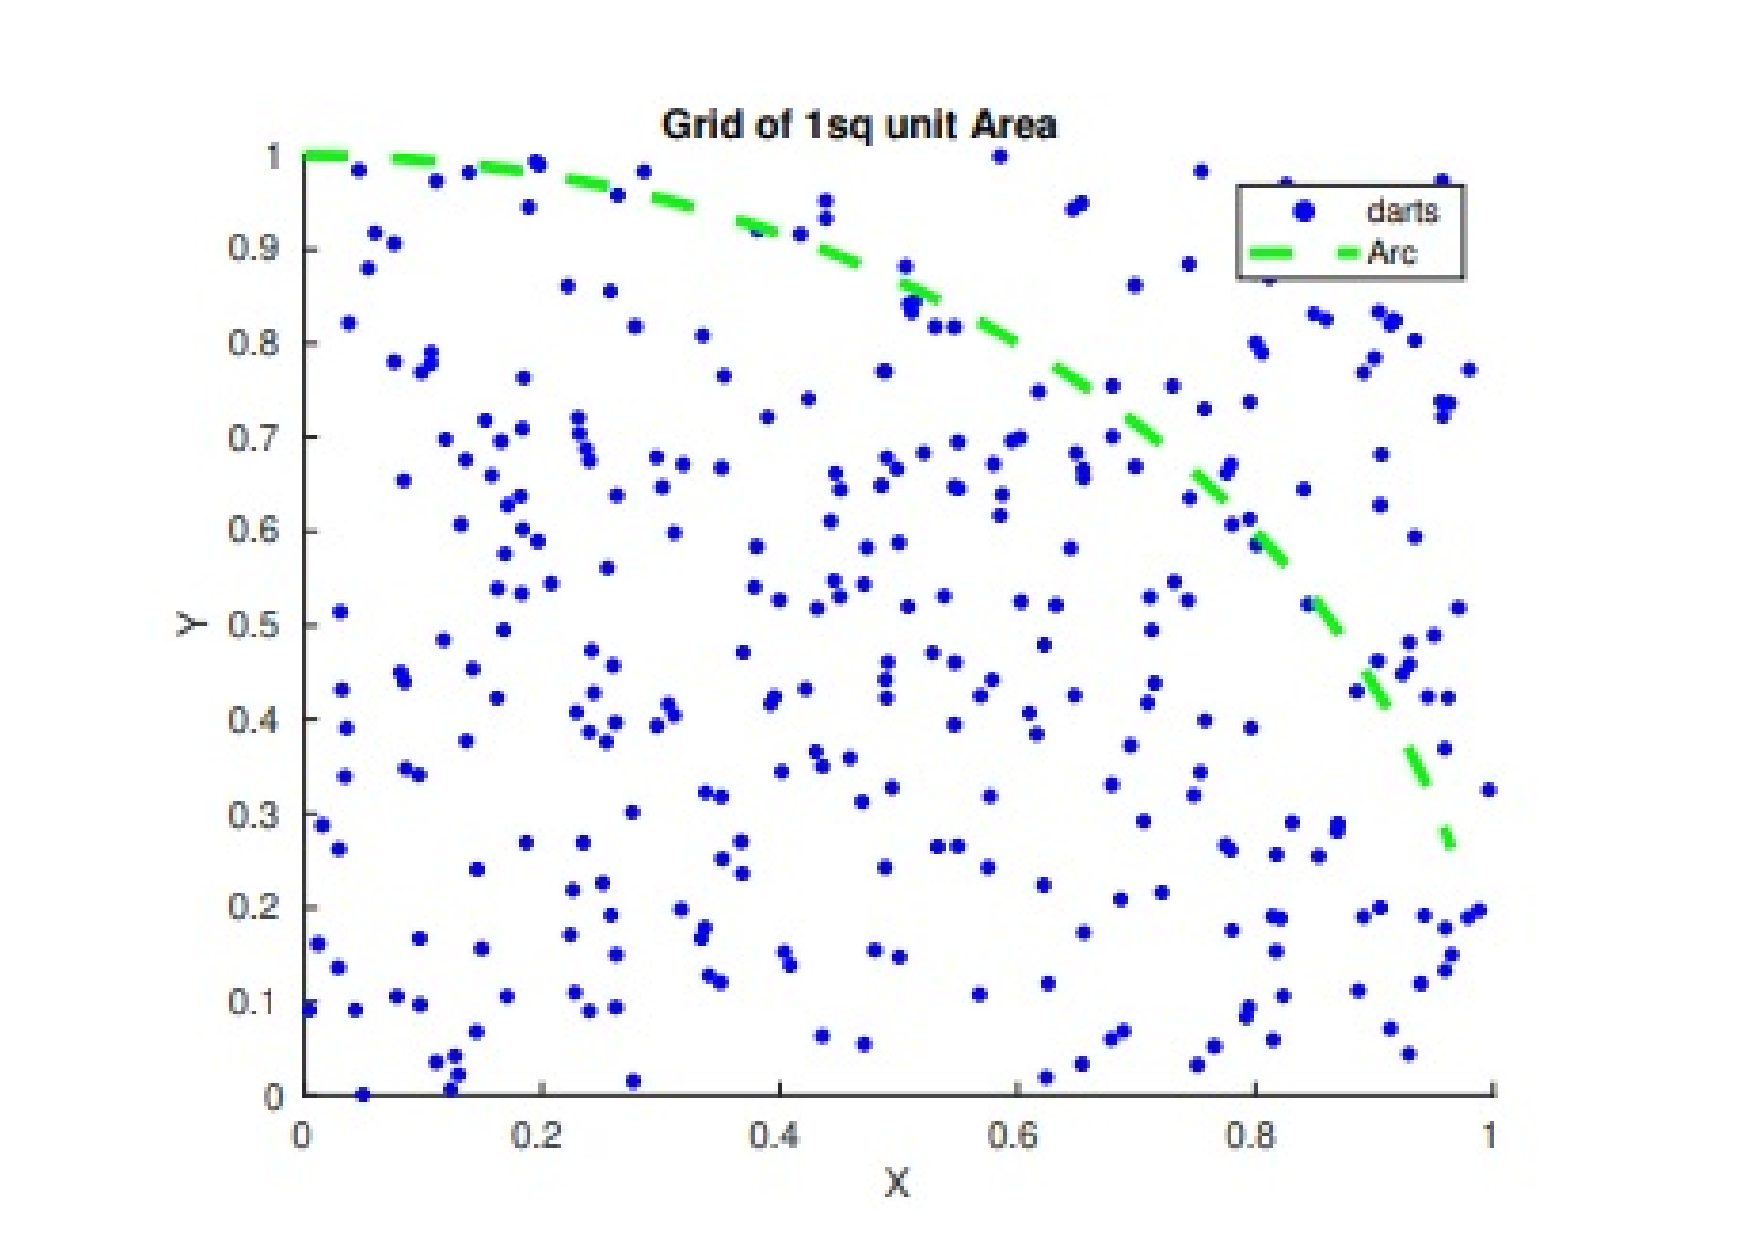
\includegraphics[width=\linewidth]{Question.pdf}
    \caption{Points on the grid denoting landed darts (n=300)}
    \label{fig:figx}
\end{figure}
  \item Iterate the sample generation to simulate the n throws of the dart uniformly in the unit square.
  \item Let $n_{arc}$ denote the number of darts that land inside the arc. Since the darts land uniformly, the ratio of number of samples inside the arc to those in the square will be proportional to their respective areas. $\pi$ can be estimated by the following equation
  \begin{align}
      \frac{n_{arc}}{n} \approx \frac{\mbox{Area of Quarter}}{\mbox{Area of Square}} = \frac{\pi}{4}
  \end{align}

\end{itemize}
Let ${{\pi}_{n}}$ denote the estimate of $\pi$ using n throws of the dart. We have
\begin{align}
    {{\pi}_{n}} = 4 * \frac{n_{arc}}{n}
\end{align}
\textbf{1(a)} \\
\begin{itemize}
    \item [(i)]Estimate $\pi$ using ${{\pi}_{n}}$ for n = $10^2$,$10^3$...$10^5$. Test out the maximum value of n, you are able to reach without any errors and tabulate your results.
    \item [(ii)]Plot ${{\pi}_{n}}$ as a function of n ($\log_{10}$ scale) \\
\end{itemize}
\textbf{1(b)} \\
\begin{itemize}
    \item [(i)] Compute the absolute error \% and tabulate along with (a)
    \item [(ii)]Plot absolute error \%  as a function of n ($\log_{10}$ scale) \\
\end{itemize}

\subsection{Approach}

In this problem, I invoke the function $srand(3141592653)$ to generate random numbers using $rand()$ for $n$ times. 
Here, I shall be taking $n$ as input from the user and compute $\pi$ from that.  
I shall use the iterative approach to find the value of $\pi$ by taking analogy to the game of darts, which is a completely random event. 

%%%%%%%%%%%%%%%%%%%%%%%%%%%%%%%%%%%%%%%%%%%%%%%%%%%%%%

\subsection{Algorithm}
In this section, I present the pseudocode/flowchart of the algorithm used to solve the problem.

The pseudocode for the summation is provided in Algorithm~\ref{alg1}.
\begin{center}
\begin{algorithm}[H]\label{alg1}

\SetAlgoLined

Input $N_{MAX}$ \\
$n_{arc} \gets 0$ \\
$n_{grid} \gets N_{MAX}$ \\
srand(3141592653)  {\\
\For {\mbox{n = 1 to $N_{MAX}$}}{
   $x \gets$ $(float)\frac{rand()}{RAND\_MAX}$ \\
   $y \gets$ $(float)\frac{rand()}{RAND\_MAX}$ \\
   $r \gets$ $\sqrt{x^2+y^2}$ \\
   n++\\
   \If {$r\leq1$}{
      $n_{arc}$ = $n_{arc}$ + 1\\
   }
  }
  ${\pi}_{n} \gets \frac{n_{arc}}{n_{grid}}*4$
}
\caption{Approximating $\pi$ }
\end{algorithm}    
\end{center}

%%%%%%%%%%%%%%%%%%%%%%%%%%%%%%%%%%%%%%%%%%%%%%%%%%%%%%
\subsection{Results}
Using $n=10^9$ random variables, we approximate the value of $\pi$ to be 3.141575 with an error of 0.000566\% which can be considered as a good estimate of $\pi$.\\
In this section, I shall plot the graphs and table that provides an overview of my findings. \\
Here, I shall plot the graphs showing the Estimate of $\pi$ vs $\log_{10}{n}$ and Error vs $\log_{10}{n}$ in Figure~\ref{fig:fig5a} and Figure~\ref{fig:fig5b} respectively. \\
The results are also summarized in Table~\ref{tab:tab2}

\begin{figure}[ht]
\begin{subfigure}{.5\textwidth}
  \centering
  % include first image
  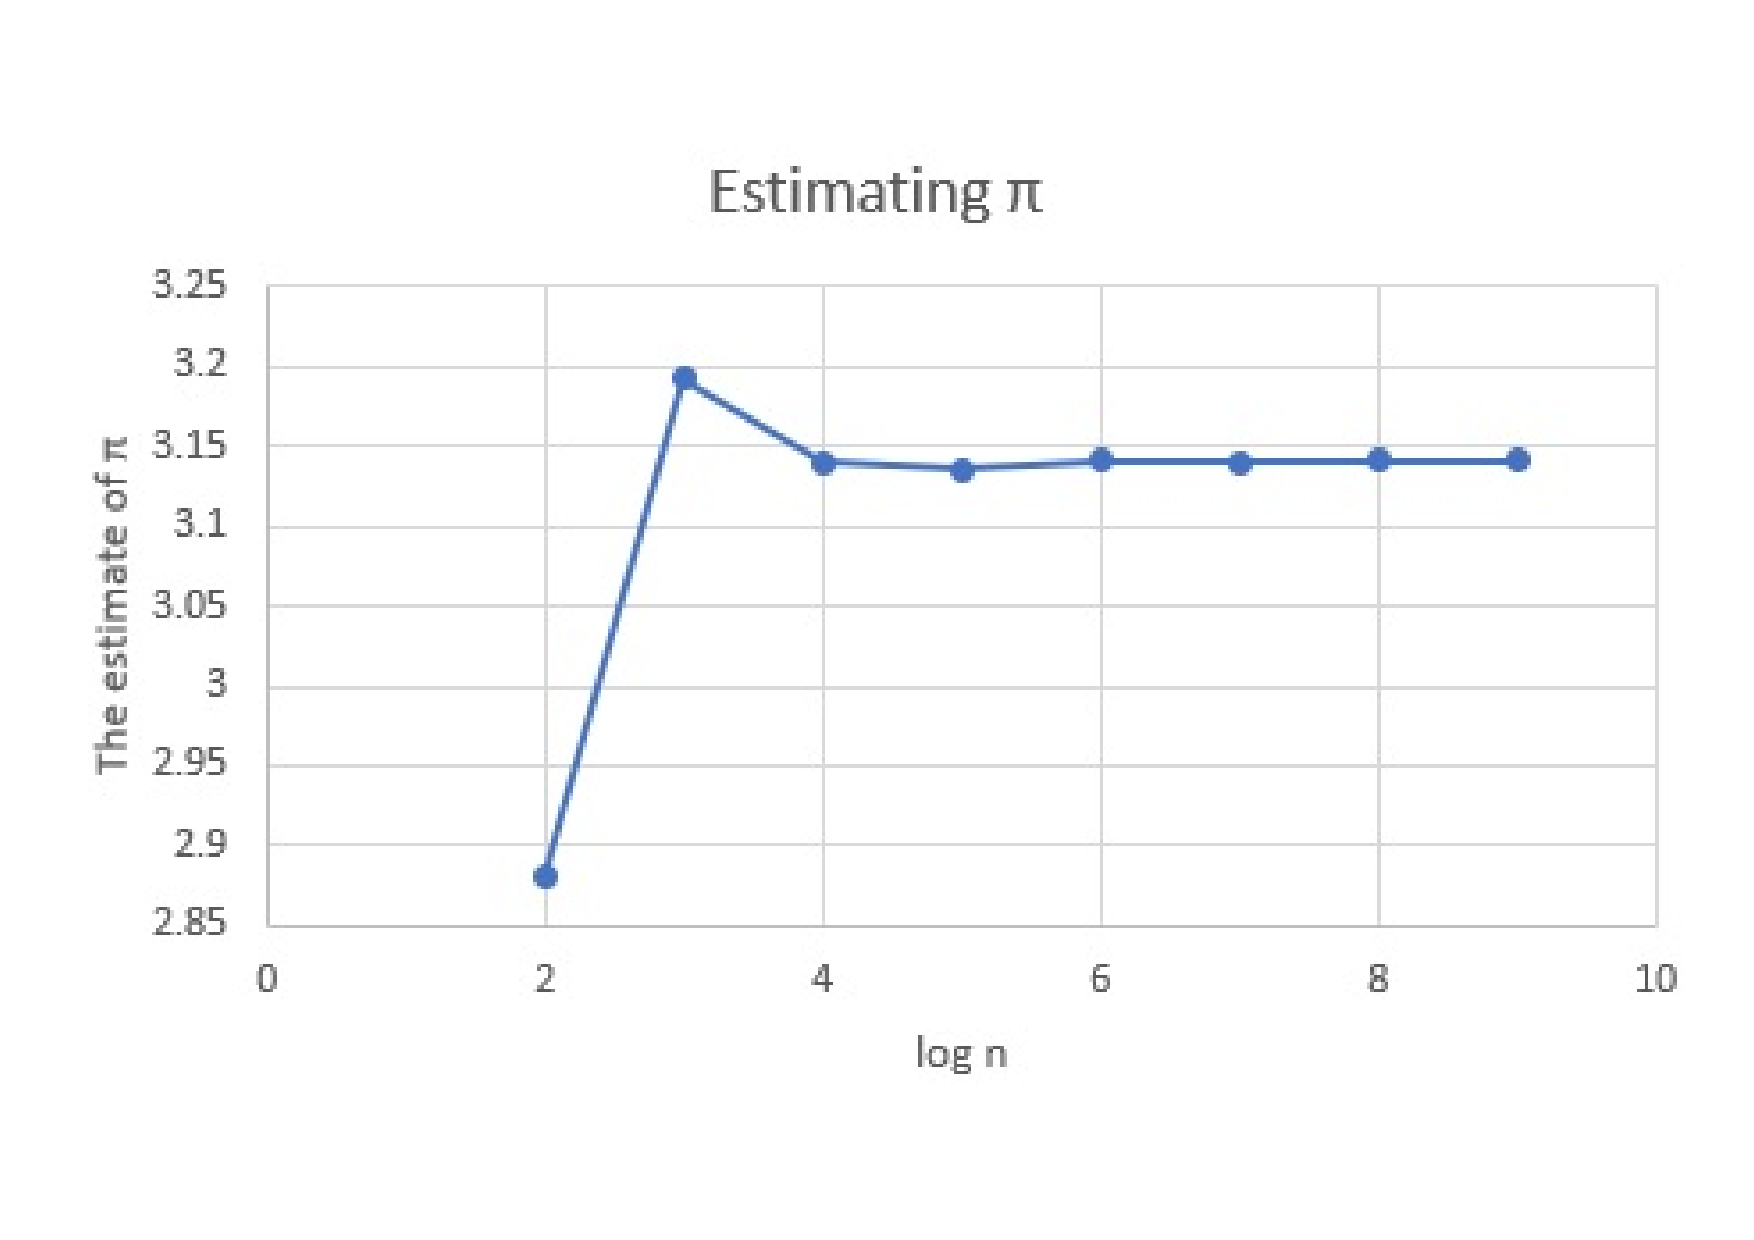
\includegraphics[width=\linewidth]{PI.pdf}
  \caption{Estimation of {$\pi$ vs $\log_{10}n$} where n is the number of random variables generated.}
  \label{fig:fig5a}
\end{subfigure}
\begin{subfigure}{.5\textwidth}
  \centering
  % include second image
  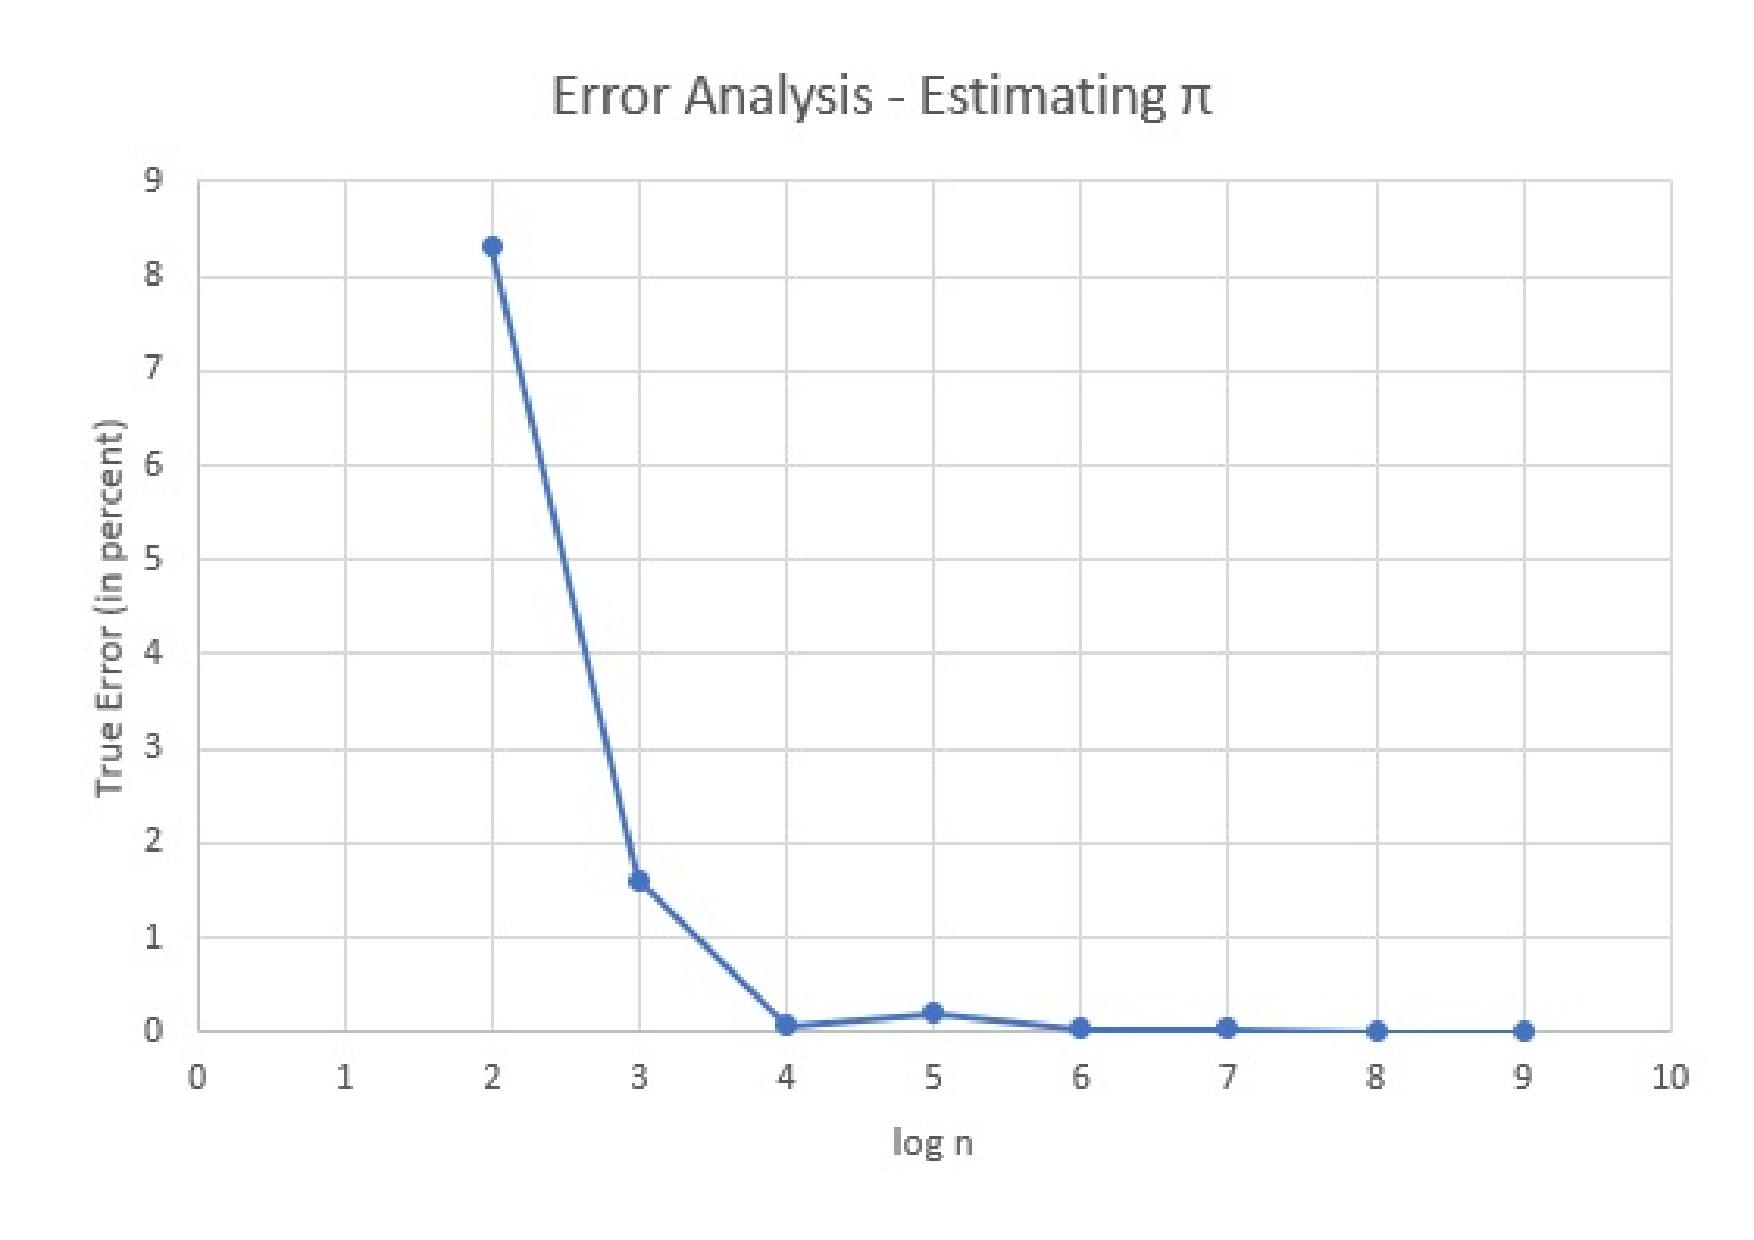
\includegraphics[width=\linewidth]{EA_PI.pdf}
  \caption{Error vs ${\log_{10}{n}}$ where n is the number of random variables generated.}
  \label{fig:fig5b}
\end{subfigure}
\caption{Estimating $\pi$}
\label{fig:q11}
\end{figure}


\begin{table}[!htb]
    \caption{Error percentage vs number of terms}
    \centering
    \begin{tabular}{ccc}
    \toprule
    \textbf{$n$}& \textbf{Estimate of $\pi$}& \textbf{Error}   \\
    \midrule
         $10^2$ & 2.880000	& 8.326749 \\
         $10^3$ & 3.192000 & 1.604513\\
         $10^4$ & 3.139600 & 0.063427 \\
         $10^5$	& 3.135440	& 0.195842 \\
         $10^6$ & 3.140652	& 0.029944 \\
         $10^7$ & 3.140396 & 0.038079 \\
         $10^8$ & 3.141517 & 0.002418 \\
         $10^9$	& 3.141575	& 0.000566 \\
    \bottomrule
    \end{tabular}
    \label{tab:tab2}
\end{table}

%%%%%%%%%%%%%%%%%%%%%%%%%%%%%%%%%%%%%%%%%%%%%%%%%%%%%%

\subsection{Inferences}

I deduce the following inferences from the Problem : 
\begin{itemize}
    \item [a.] The decline in the error percentage, even in the logarithmic scale, as a function of $n$ in Figure~\ref{fig:fig5b} shows that the estimated value of $\pi$ converges to the true value of $\pi$ as we increase the number of random variables. In principle, as n goes to $\infty$, the estimated value of $\pi$ shall approach the true value of $\pi$, and thus reduce the error percentage to \textit{zero}
    \item [b.] The random numbers generated are not truly \emph{random} but are \emph{pseudo-random} as they are produced by an algorithm running on the computer. 
    \item [c.] Our assumption of a uniform random variable $X$ does not seem absolutely correct as our computer can generate only discrete numbers upto a certain precision. Howsoever, it can be considered as a \textbf{good approximation}.
    \item [d.]The error propagates as $\frac{1}{\sqrt{n}}$ where n is the number of random variables generated. Though, it does not seem apparent from the Table~\ref{tab:tab2}, it appears to be correct for larger n.
    \item [e.] As the number of random variables (assumed uniform) increase, we gradually approach $\pi$. The online compiler is successfully able to iterate for $10^9$ iterations, post which we are able to estimate $\pi$ to be 3.141575 with an error of 0.000566 \%.
    \item [f.] Here I have taken n as input from the user each time. Howsoever, if we use a loop without taking input from the user, the answer $\pi$ we obtain differ. This is because srand() is invoked only once in the latter, and srand() is invoked each time the user enters the value of n. In the former case, that is, the method which I have used shall give the same output regardless of the order of input, that is, 10,100,1000 gives the same output as 1000,100,10 or any other permutation. In the loop case, this is not true generally. 
    \item [f.] This method of estimating $\pi$ is termed as \textbf{Monte Carlo's Method.}
\end{itemize}

%%%%%%%%%%%%%%%%%%%%%%%%%%%%%%%%%%%%%%%%%%%%%%%%%%%%%%

\subsection{Code}
The code used for the experiments is mentioned in Listing~\ref{listing:1}. 

\inputminted[breaklines,
 mathescape,
 linenos,
 numbersep=5pt,
 frame=single,
 numbersep=5pt,
 xleftmargin=0pt]{c}{A2P1.c}
 \captionof{listing}{Code snippet used in the Problem.}
\label{listing:1}

%%%%%%%%%%%%%%%%%%%%%%%%%%%%%%%%%%%%%%%%%%%%%%%%%%%%%%

\subsection{Contributions}
In the above problem, \textit{my original contributions} are - 
\begin{itemize}
    \item Designing of the Algorithm and Code
    \item Plotting of the graph on Google Sheets and MS Excel
    \item Analysis of True Error
    \item Tabulation of Results and Errors
    \item Drawing conclusions by looking at the Result obtained and Error Analysis.
    \item Wri
\end{itemize}

%%%%%%%%%%%%%%%%%%%%%%%%%%%%%%%%%%%%%%%%%%%%%%%%%%%%%%

\subsection{Alternate Methods}
\begin{itemize}
    \item [1.]The \textbf{Monte Carlo Method} provides a good estimate of $\pi$, but for applications and programs requiring higher precision and accuracy, we cannot use the \textbf{Monte Carlo Method} due to its higher time complexity and comparatively lower accuracy. 
    \item[2.] The \textbf{Chudnovsky Algorithm based on Ramanujam's Formula} provides a quicker estimate of $\pi$, (\emph{Reference :} \href{https://en.wikipedia.org/wiki/Chudnovsky_algorithm}{Chudnovsky Algorithm} ) estimating upto millions and billions of digits within minutes.
    \item [3.] Since many websites and calculators provide the value of $\pi$ upto 15 or 20 digits, in applications or programs requiring $\pi$ upto a higher precision, or for the general use of Mathematicians, a good programming approach would be to define a macro and using the same as shown in the example below : \\ 
    \begin{center}
    \boxed{\mbox{\# define PI 3.141592653}}
    \end{center}
\end{itemize}

%%%%%%%%%%%%% END OF QUESTION 1 %%%%%%%%%%%%%%%%%%%%
\newpage
\section{Problem 2}
Generate samples from a standard normal distribution from uniform random samples, using \emph{the Box-Muller transform.}
\begin{itemize}
    \item Generate two sets of uniform distribution (say $U_1$ and $U_2$) in [0, 1).
    \item Obtain a standard exponential random variable from $U_1$ 
    \begin{equation}
        E = - \log(U_1)
    \end{equation}
    \item Generate the two sets of standard normal variables using the below transform : 
    \begin{equation}
        X = \sqrt{E} \cos{2 \pi U_2} 
    \end{equation}
    \begin{equation}
        Y = \sqrt{E} \sin{2 \pi U_2} 
    \end{equation}
    \item X and Y will be independent zero-mean unit variance Gaussian random variables (or standard Normal random variables).
\end{itemize}
\textbf{2(a)} \\
Generate n = 100, 1000, 10000 samples of X defined above, use $srand(0)$ as the seed for comparison of outputs. \href{https://www.onlinegdb.com/online_c_compiler}{(onlinegdb)}
\begin{itemize}
    \item [(i)] Plot histograms for the samples generated \\
\end{itemize}
\textbf{2(b)} \\
\begin{itemize}
    \item [(i)] Plot the \href{https://en.wikipedia.org/wiki/Empirical_distribution_function}{Empirical Distribution Function(EDF)} of X (to approximate the Cumulative Distribution Function) for values of n = 10, 100, 1000. You can choose the x-axis range to be [−4, 4], since most of the probability mass of the standard normal lies in this interval.
    \item [(ii)]Compute the empirical estimate for Erf(1) and Erf(2) for n = 10000 samples, as the fraction of the generated samples that are less than or equal to 1 (and 2 respectively). Equivalently, these are just the EDF values at 1 and 2 respectively.
\end{itemize}

\subsection{Approach}

In this problem, I invoke the function $srand(0)$ as a seed to generate random numbers using $rand()$ for $n$ times on \href{https://www.onlinegdb.com/online_c_compiler}{Online GDB }. \\
I shall use the iterative approach to find the Gaussian Distribution of $n$ Random variables and plot Histograms and Empirical Distribution Function (EDF) for \emph{n = 100, 1000 and 10000}. \\ 
%%%%%%%%%%%%%%%%%%%%%%%%%%%%%%%%%%%%%%%%%%%%%%%%%%%%%%

\subsection{Algorithm}
In this section, I present the pseudocode/flowchart of the algorithm used to solve the problem.

The pseudocode for the summation is provided in Algorithm~\ref{alg2}.
\begin{center}
\begin{algorithm}[H]\label{alg2}

\SetAlgoLined

Input $N_{MAX}$ \\
srand(0) \\
\For {\mbox{n = 1 to $N_{MAX}$}}{
   $U_1 \gets$ $(float)\frac{rand()}{RAND\_MAX}$ \\
   $U_2 \gets$ $(float)\frac{rand()}{RAND\_MAX}$ \\
   $E \gets \log{\frac{1}{U_1}}$ \\
   $x \gets$ $\sqrt{E} \cos{2\pi U_2}$ \\
   $y \gets$ $\sqrt{E} \sin{2\pi U_2}$ \\
   Store x and y
   }

 \caption{Box Muller Transform}
\end{algorithm}    
\end{center}

%%%%%%%%%%%%%%%%%%%%%%%%%%%%%%%%%%%%%%%%%%%%%%%%%%%%%%
\subsection{Results}
In this section, I shall plot the graphs and the table that provide an overview of my observation. \\

Now, I plot the histogram showing frequency against the random variable in contention in Figure~\ref{fig:q21}, Figure~\ref{fig:q22} and Figure~\ref{fig:q23}. \\

\begin{figure}[ht]
\begin{subfigure}{.5\textwidth}
  \centering
  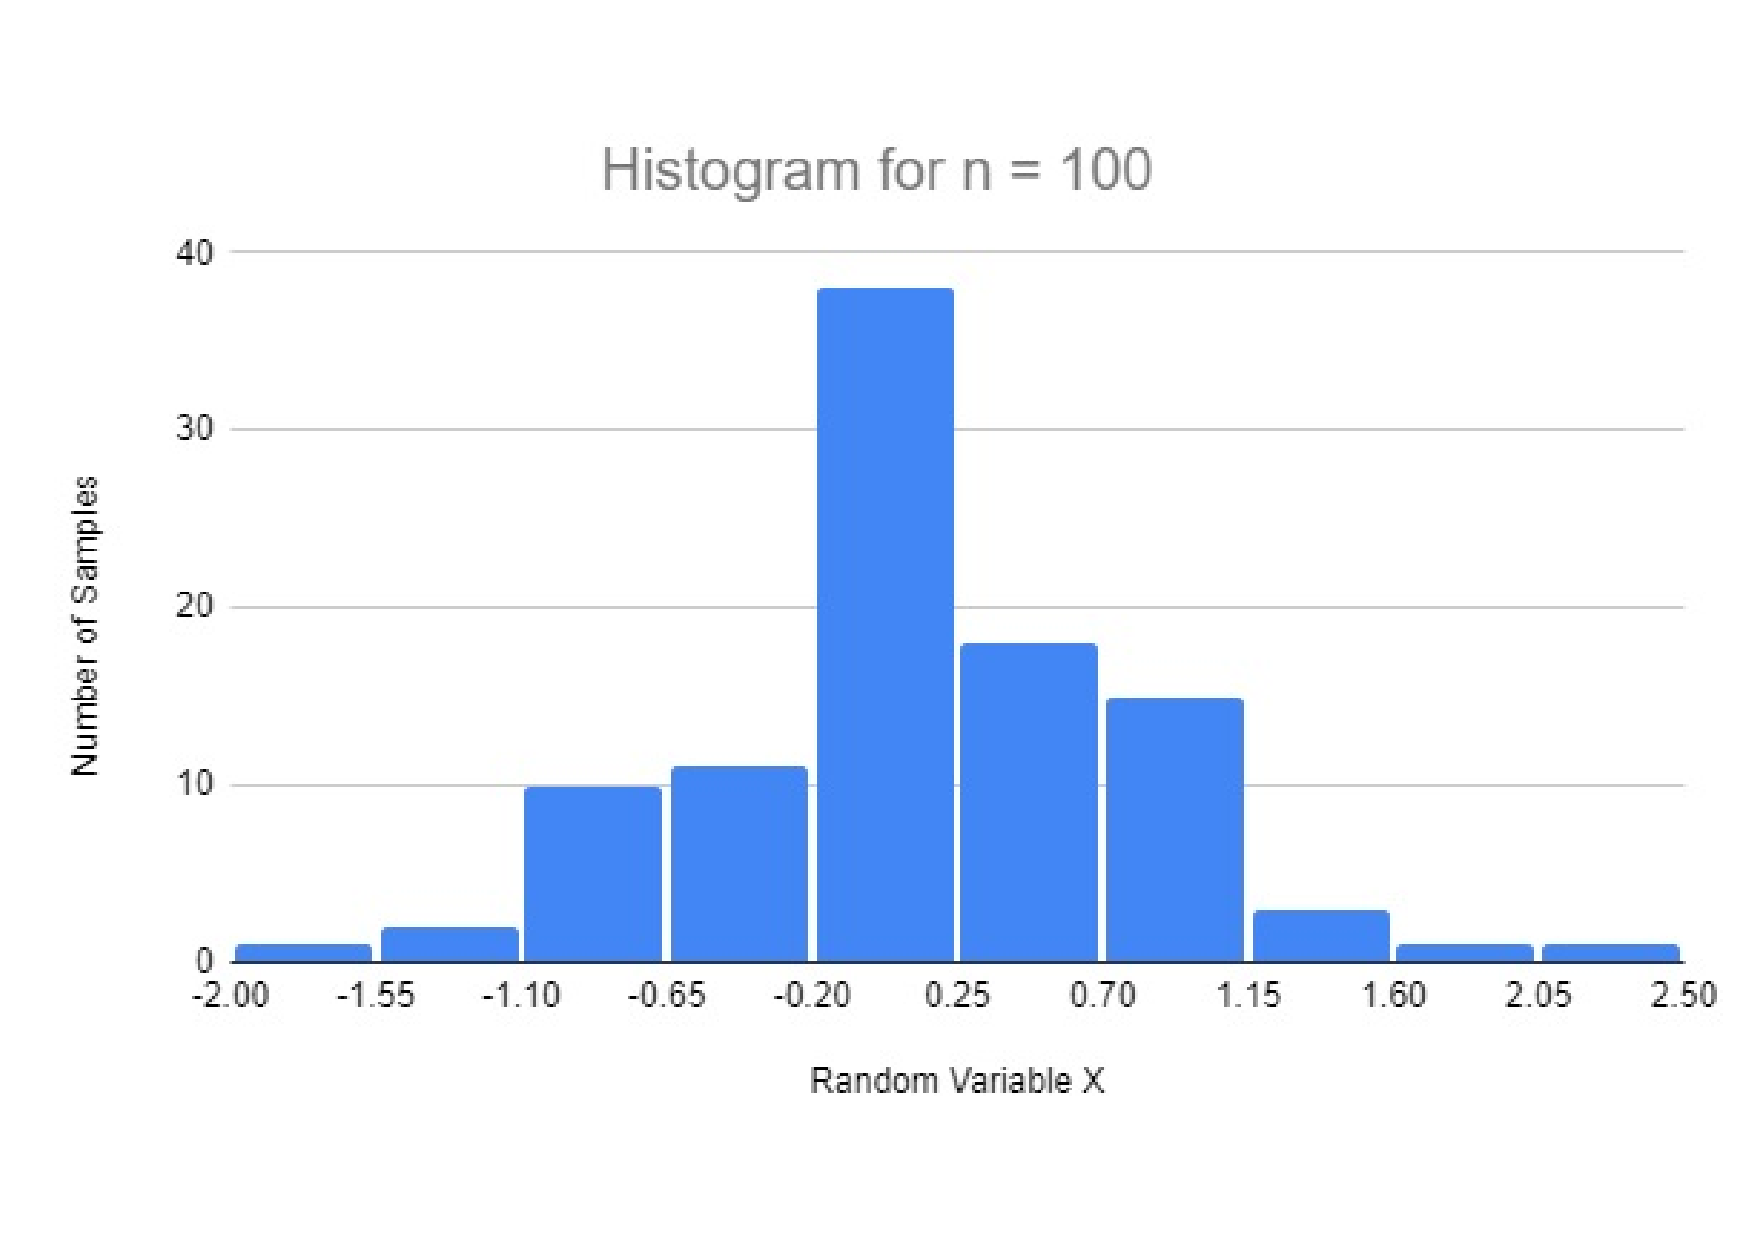
\includegraphics[width=\linewidth]{HIS100.pdf}
  \caption{Histogram showing frequency of a random variable generated $n=100$ times. }
  \label{fig:q21}
\end{subfigure}
\begin{subfigure}{.5\textwidth}
  \centering
  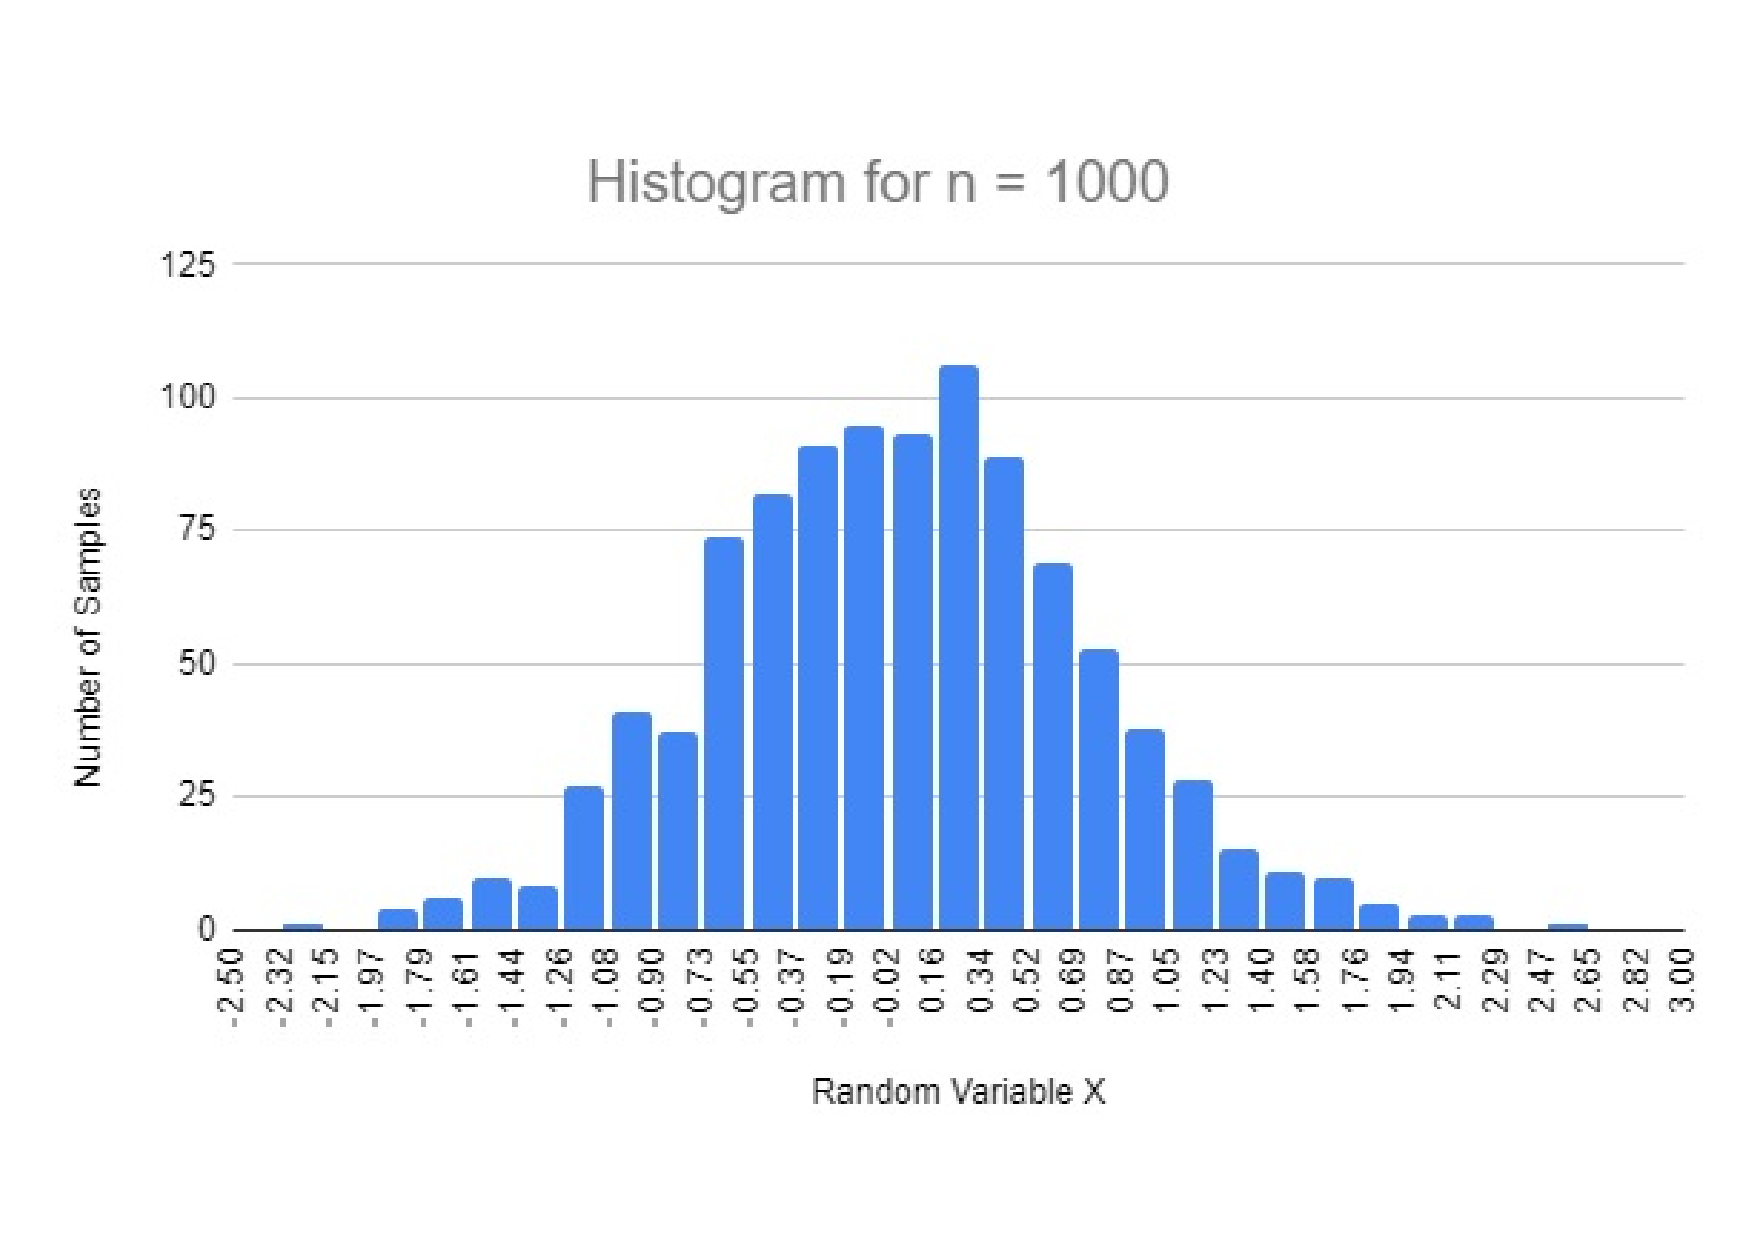
\includegraphics[width=\linewidth]{HIS1000.pdf}
  \caption{Histogram showing frequency of a random variable generated $n=1000$ times. }
  \label{fig:q22}
\end{subfigure}
\begin{subfigure}{.5\textwidth}
  \centering
  \begin{center}
  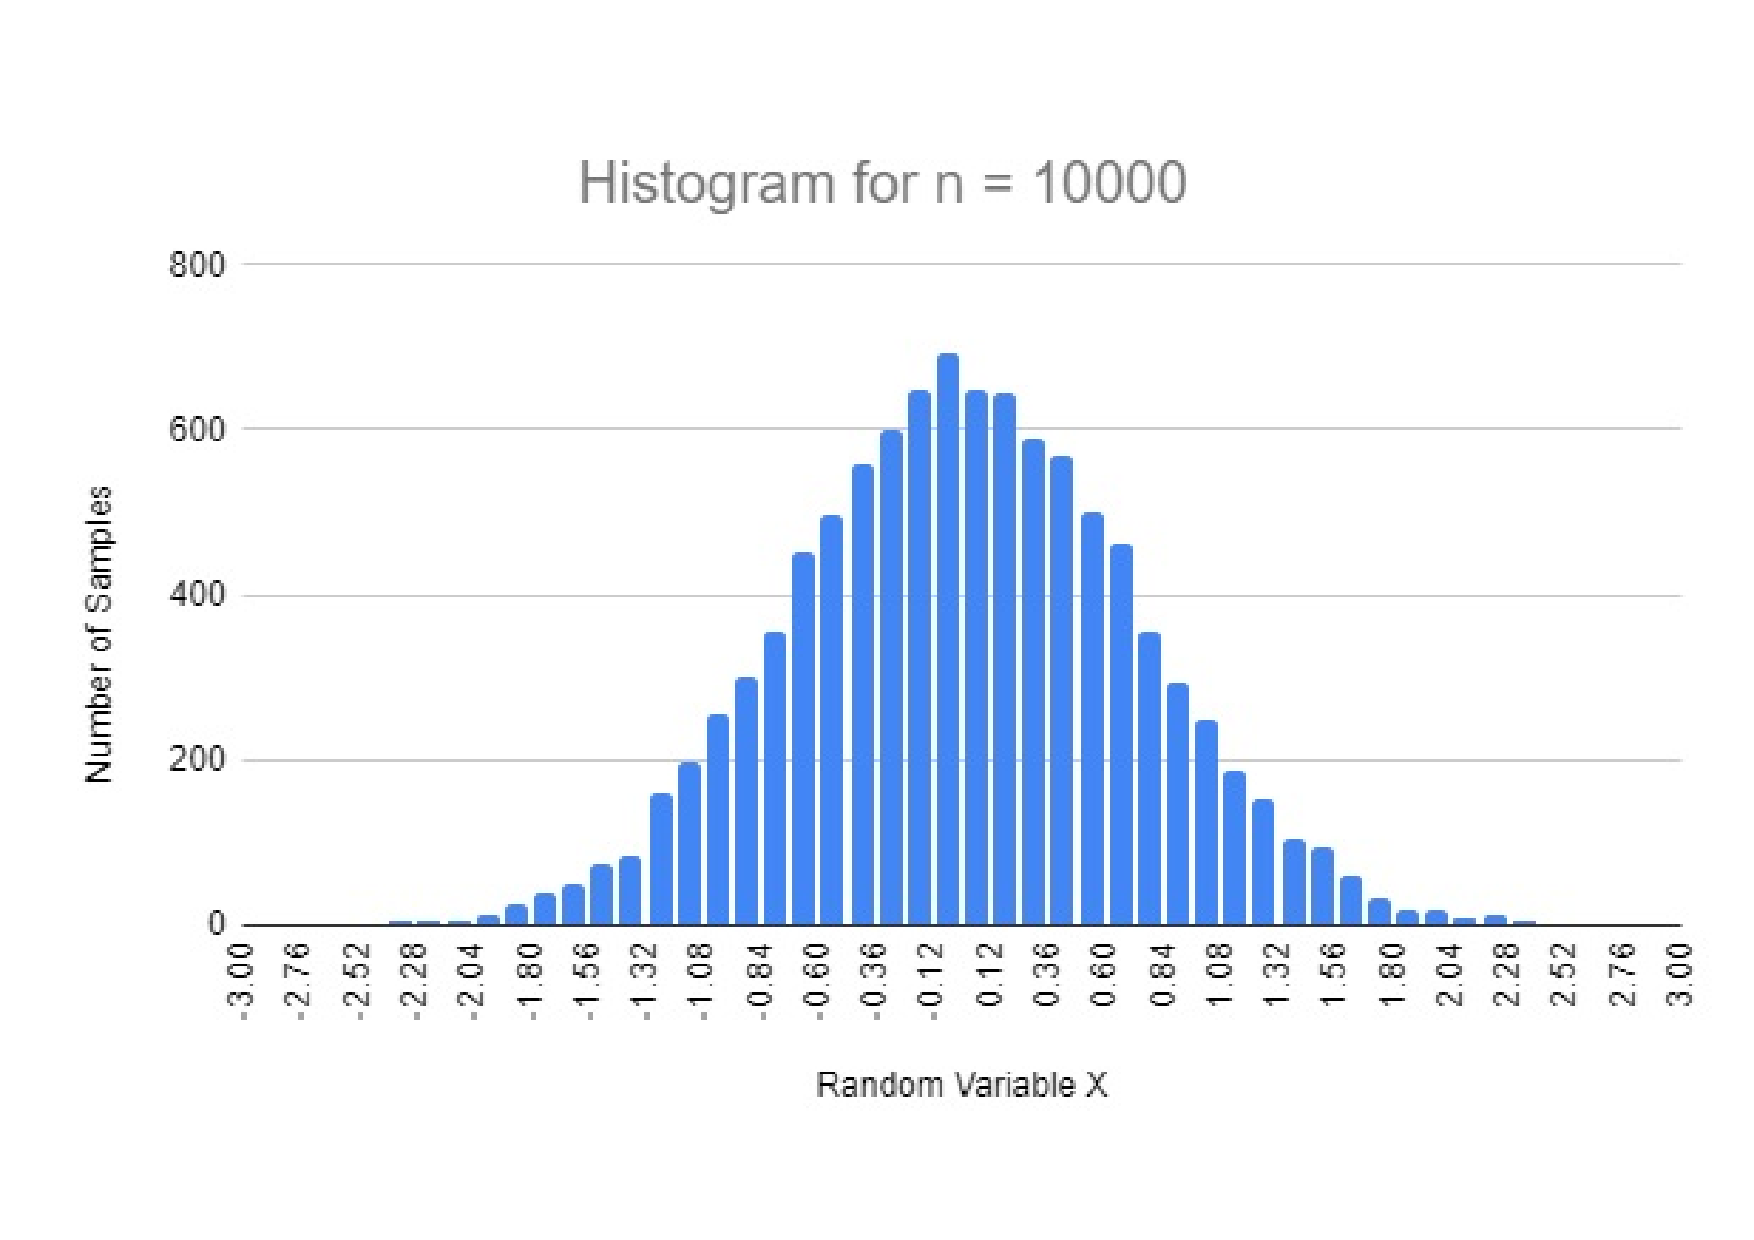
\includegraphics[width=\linewidth]{HIS10000.pdf}
  \end{center}
  \caption{Histogram showing frequency of a random variable generated $n=10000$ times. }
  \label{fig:q23}
\end{subfigure}
\caption{Histogram showing frequency of a random variable generated $n$ times.}
\label{fig:q2}
\end{figure}

Here, I plot the Empirical Distribution Function (EDF) of X plotted against random variable X for $n$ iterations. It is shown in Figure~\ref{fig:q31}, Figure~\ref{fig:q32} and Figure~\ref{fig:q33}.\\

\begin{figure}[ht]
\begin{subfigure}{.5\textwidth}
  \centering
  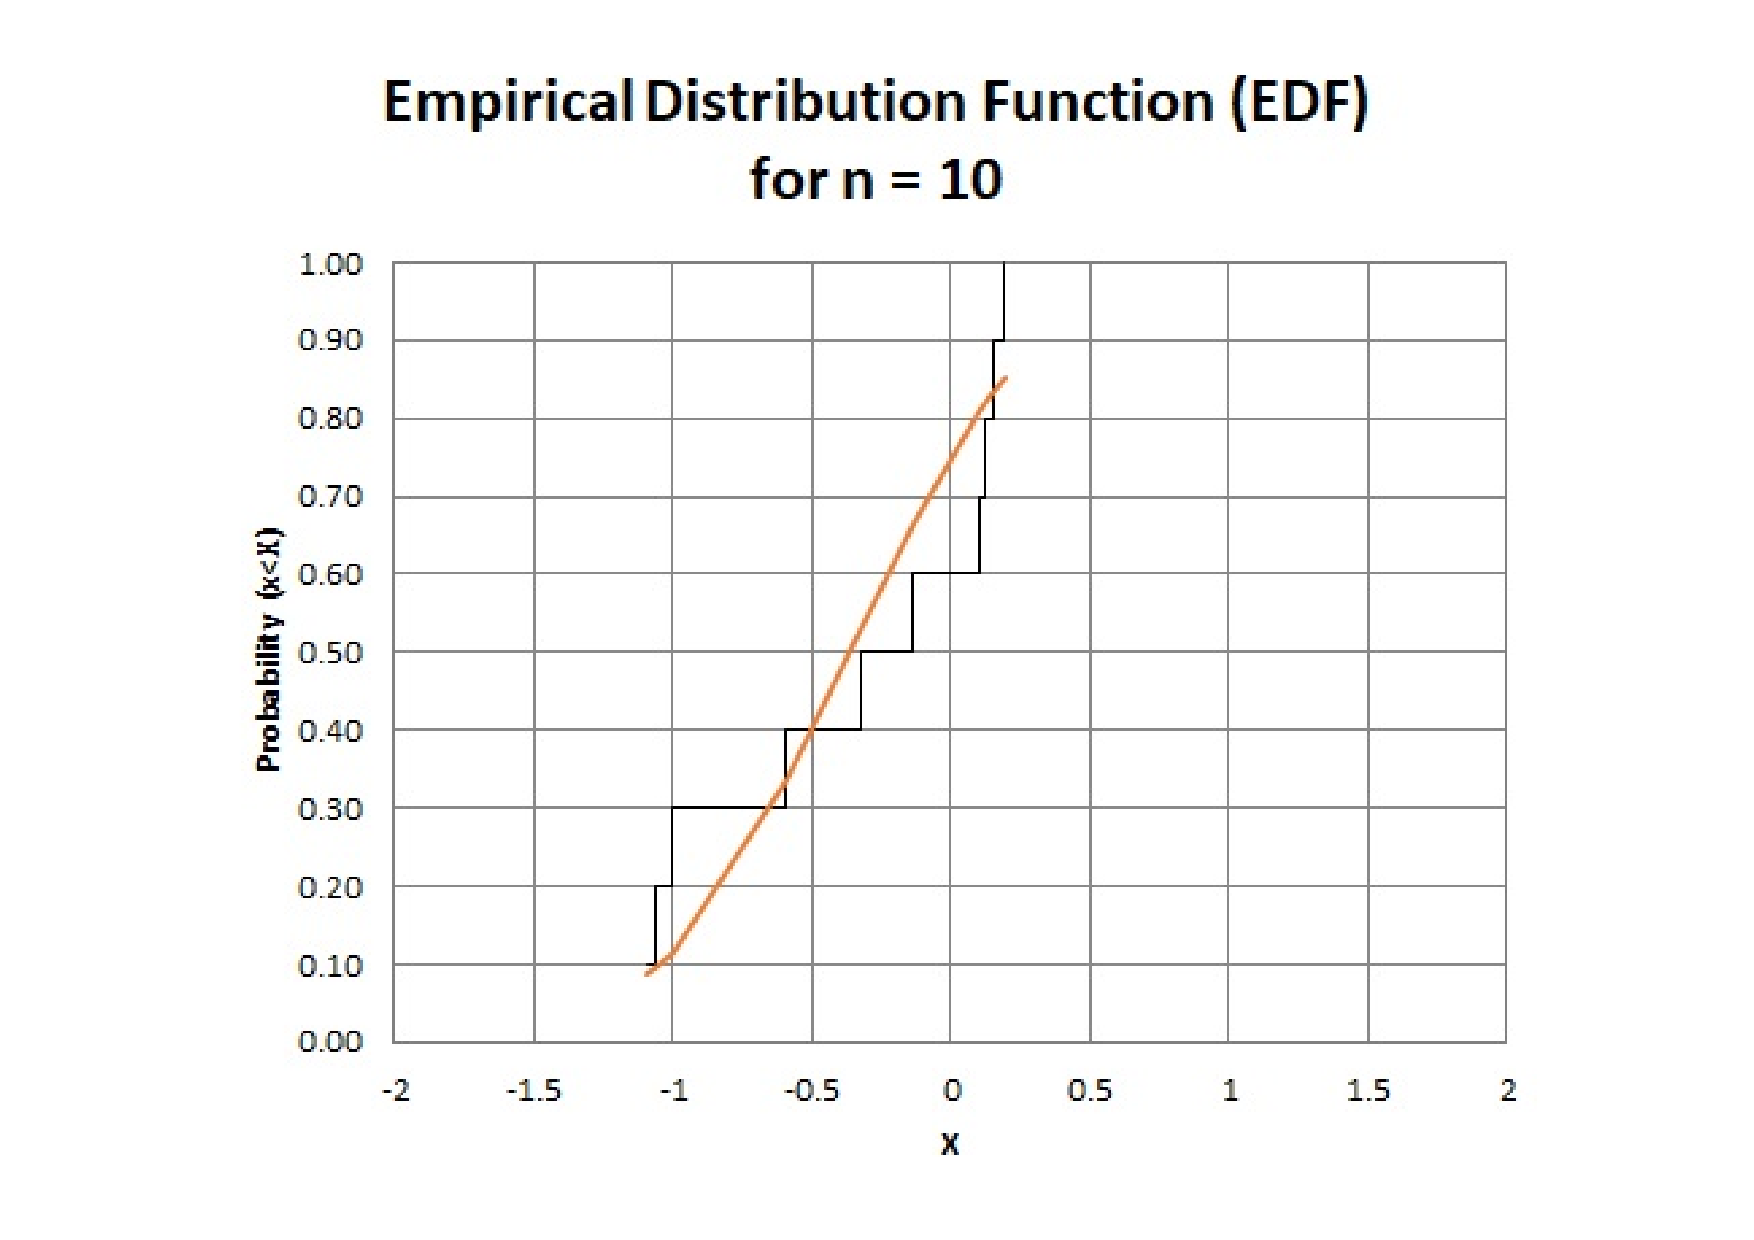
\includegraphics[width=\linewidth]{EDF10.pdf}
  \caption{Empirical Distribution Function (EDF) of X plotted against random variable X for $n=10$ samples. }
  \label{fig:q31}
\end{subfigure}
\begin{subfigure}{.5\textwidth}
  \centering
  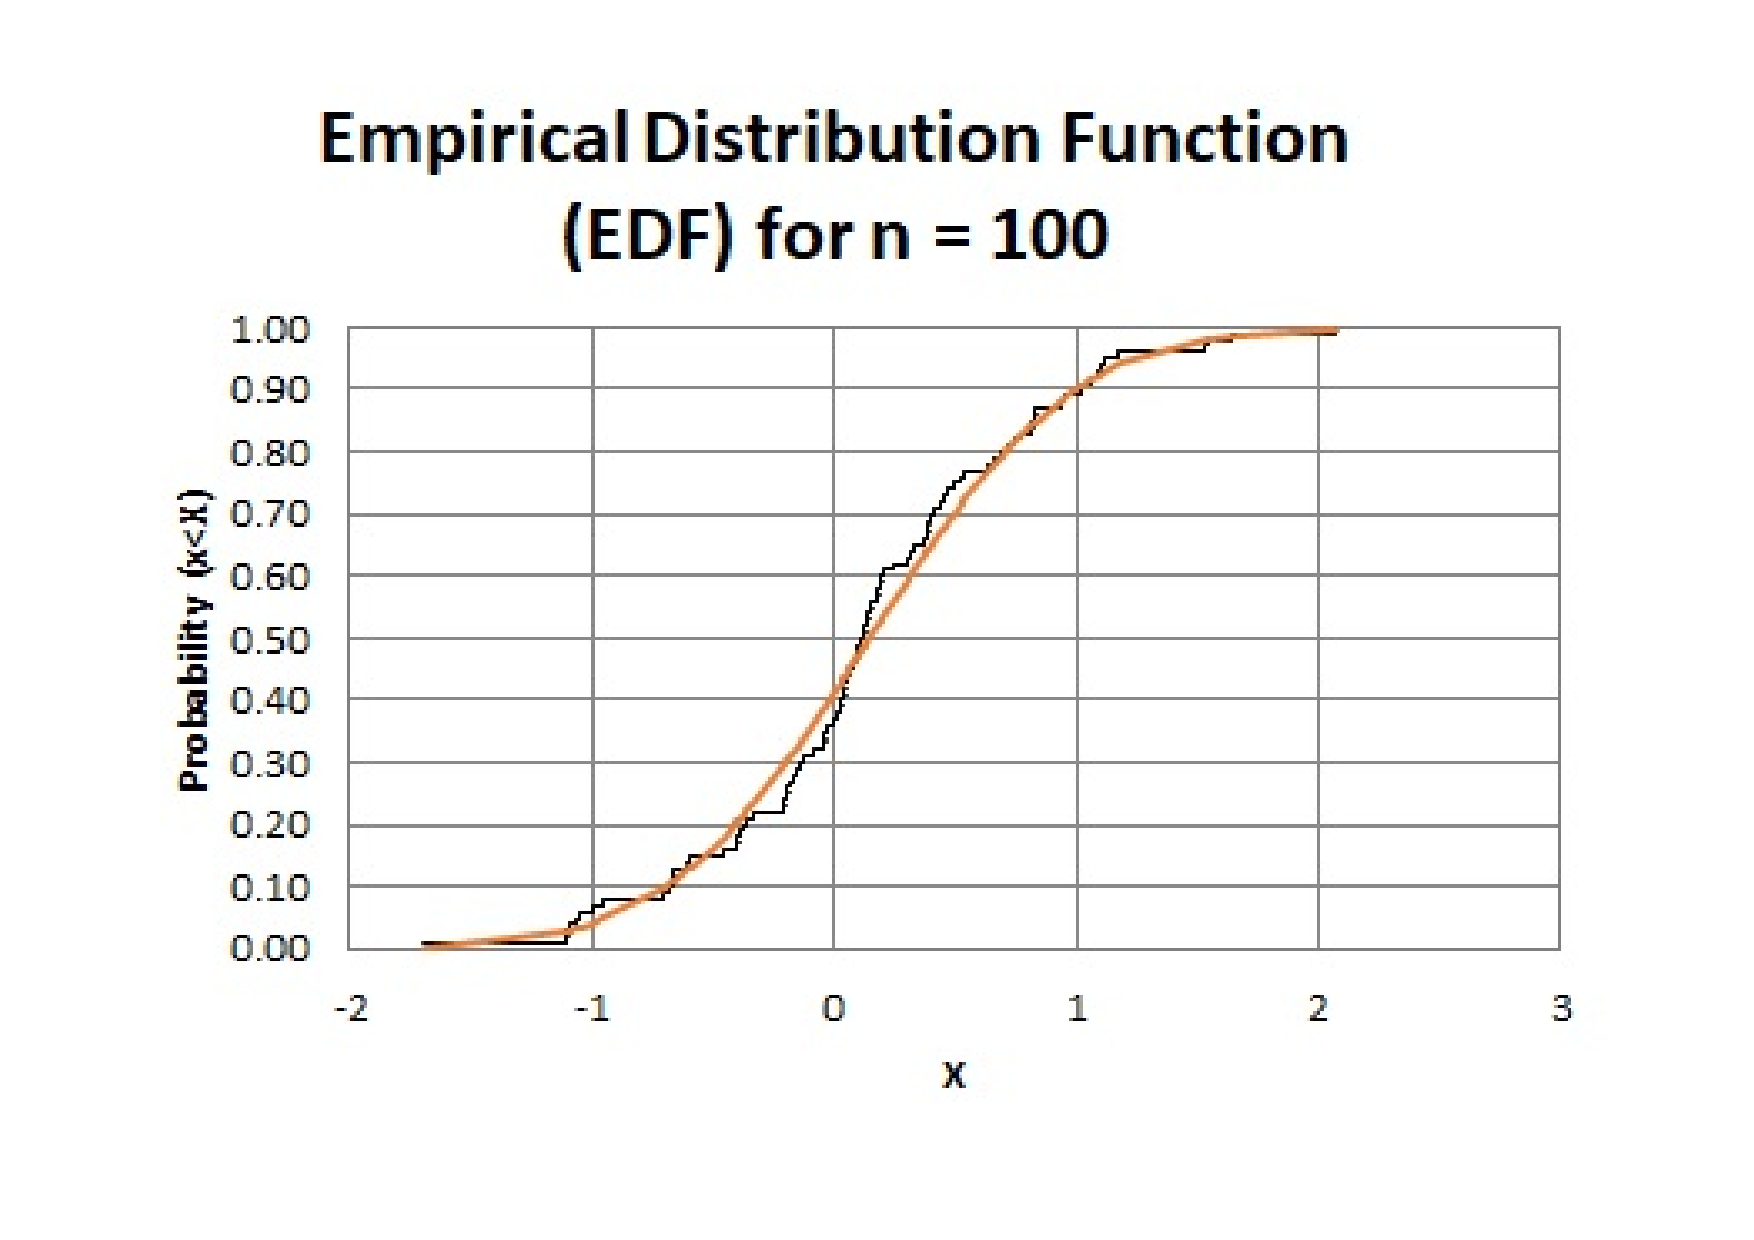
\includegraphics[width=\linewidth]{EDF100.pdf}
  \caption{Empirical Distribution Function (EDF) of X plotted against random variable X for $n=100$ samples. }
  \label{fig:q32}
  \end{subfigure}
  \begin{subfigure}{.5\textwidth}
  \begin{center}
  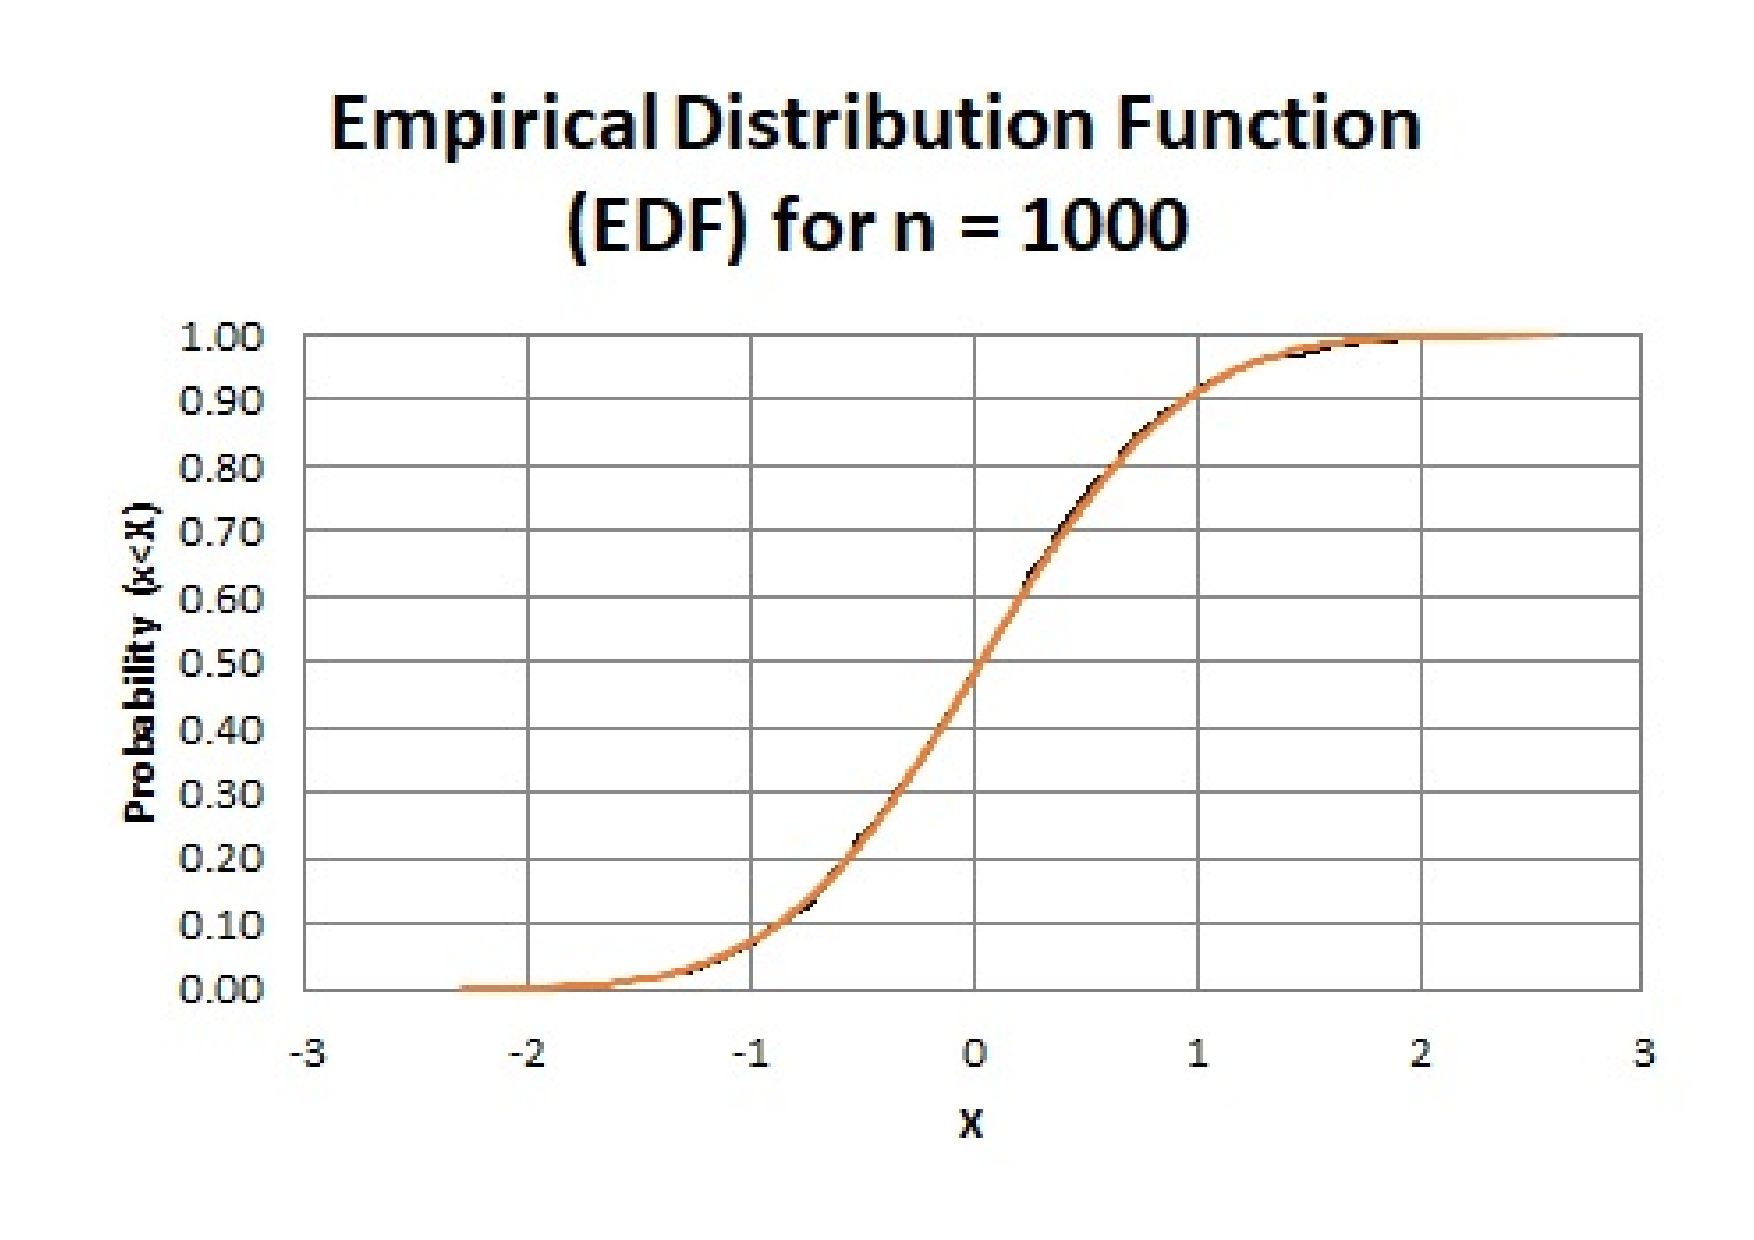
\includegraphics[width=\linewidth]{EDF1000.pdf}
  \end{center}
  \caption{Empirical Distribution Function (EDF) of X plotted against random variable X for $n=1000$ samples. }
  \label{fig:q33}
\end{subfigure}
\caption{Empirical Distribution Function (EDF) showing probability (x $\leq$ X) of a random variable X generated $n$ times.}
\label{fig:q3}
\end{figure}

As seen from the graph for $n=10000$ in Figure~\ref{fig:q4}, the values of ERF(1) and ERF(2) are the values of the EDF at 1 and 2 respectively. I deduce the following - \\
\begin{itemize}
    \item [1.] ERF(1) = EDF(1) = 0.9160
    \item [2.] ERF(2) = EDF(2) = 0.9973
\end{itemize}
\begin{figure}
    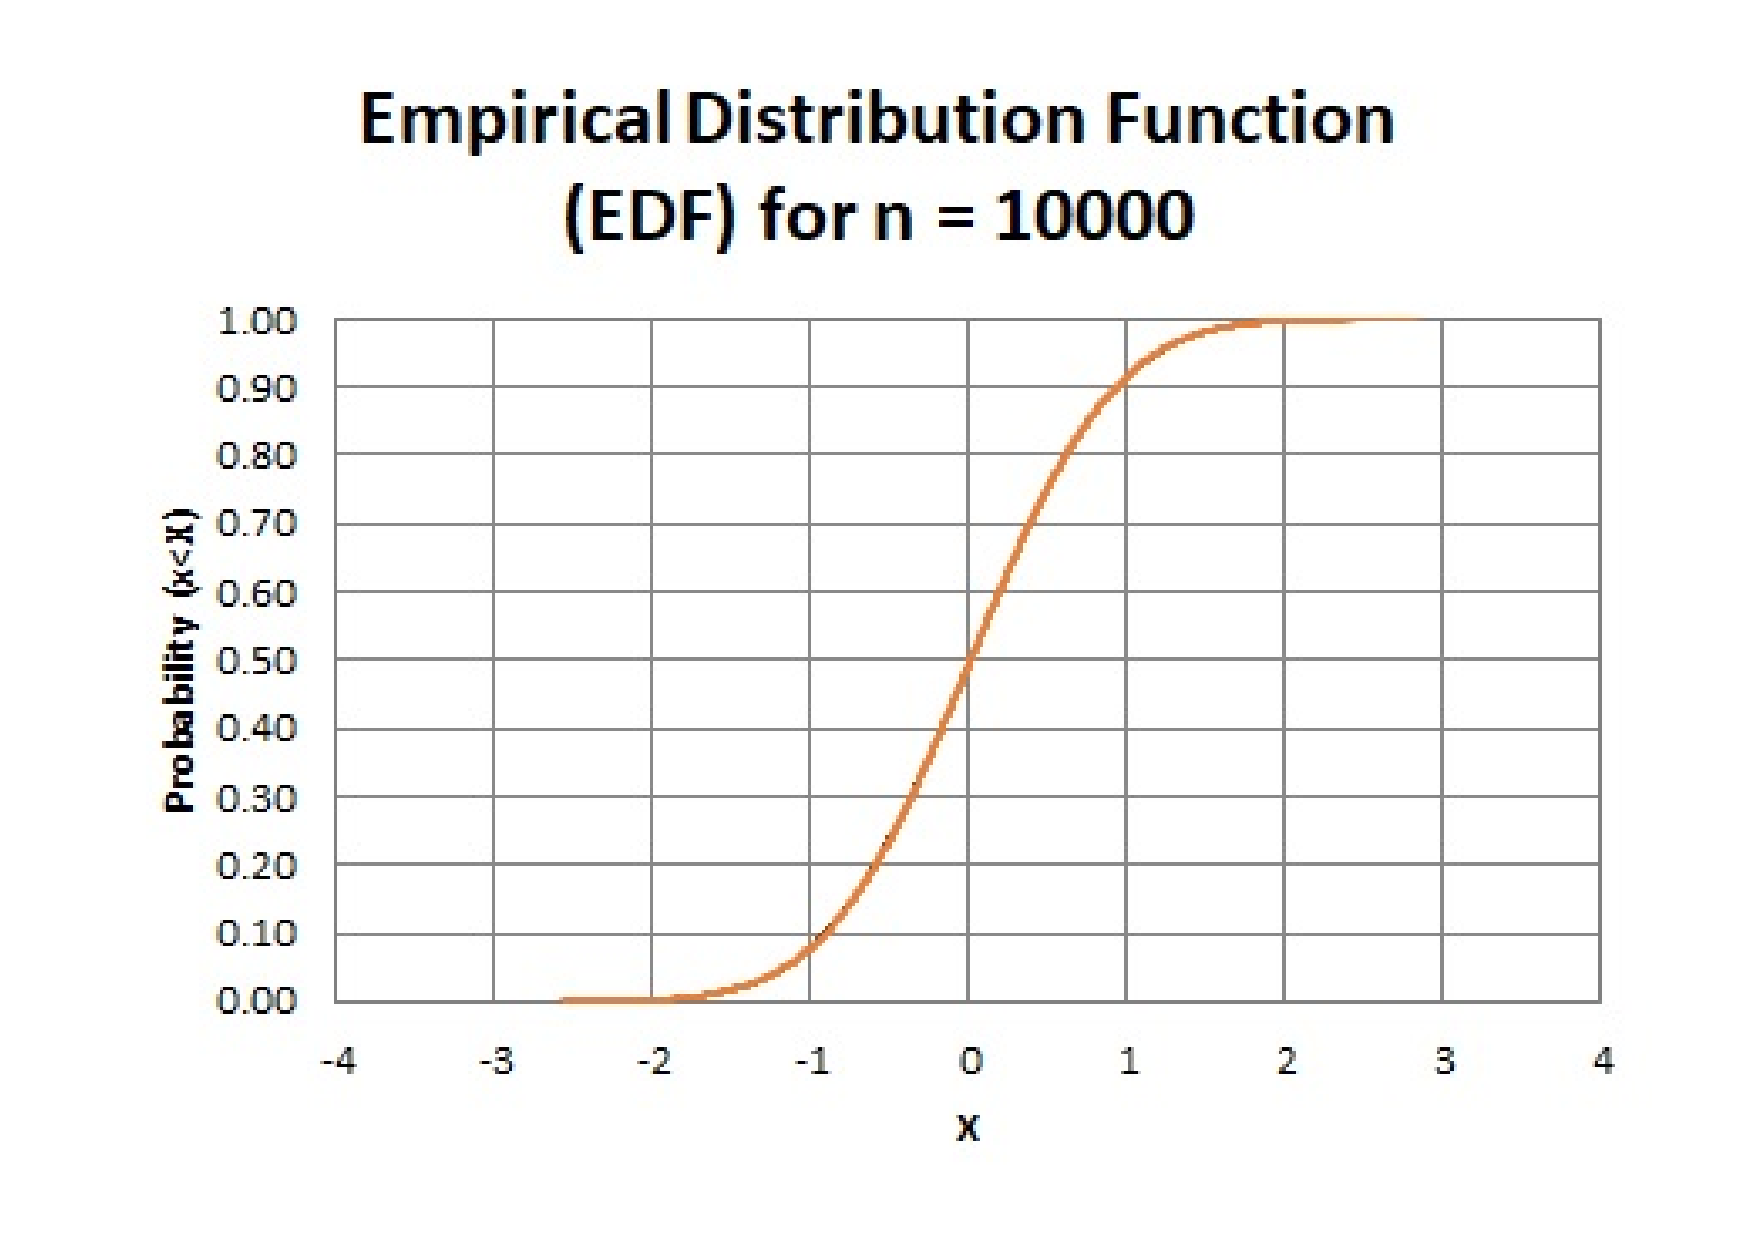
\includegraphics[width=\linewidth]{EDF10000.pdf}
    \caption{Empirical Distribution Function (EDF) showing Probability (x $\leq$ X) against Random Variable X}
    \label{fig:q4}
\end{figure}
%%%%%%%%%%%%%%%%%%%%%%%%%%%%%%%%%%%%%%%%%%%%%%%%%%%%%%

\subsection{Inferences}

I deduce the following inferences from the problem :
\begin{itemize}
    \item [a.] We see that the Histogram takes up a Gaussian distribution as we increase $n$, the number of random numbers generated using the \textbf{Box Muller Transform.}
    \item [b.] The Empirical Distribution Function (EDF) line converges to the Cumulative Distribution Function (CDF) as the number of random variables $n$ increase. This is totally surprising as a continuous and non-differentiable function (EDF) converges to a continuous and smooth function (CDF) and \emph{vice-versa.}
    \item [c.] The random numbers generated are not truly \emph{random} but are \emph{pseudo-random} as they are produced by an algorithm running on the computer. 
     \item [d.] Our assumption of uniform random variables $U_1$ and $U_2$ as well as the Gaussian pair $X$ and $Y$ does not seem absolutely correct as our computer can generate only discrete numbers upto a certain precision. Howsoever, it can be considered as a \textbf{good approximation}.
     \item [e.] In principle, as we extend the number of random variables $n$ to $\infty$, the Histograms would converge to a well known Gaussian Distribution. 
     \item [f.] The actual values of ERF(1), ERF(2) and ERF(4) as computed by a calculator are 0.8427, 0.9953 and 0.9999 respectively. However, the code produces values corresponding to ERF(1), ERF(2) and ERF(4) as 0.9160, 0.9973 and 1 respectively. This seems quite off the actual answer. This can be explained by the fact that the number of random values $n$ are small, thus the ERF values do not converge to the ones as hinted out by a calculator. Another plausible explanation to the same would be of the finite precision and accuracy of the computing machine which can store and reproduce only a fixed number of digits. Moreover, a computer works in the digital domain where numbers are discrete, where as the ERF values generated by a calculator work on continuous distributions. 
     \item [g.] Another interesting inference is that as the number of random variables $n$ increases, the ERF(x) reduces. In principle, as $n$ would approach $\infty$, the ERF(x) would converge to its actual value as computed by a calculator. 
\end{itemize}

%%%%%%%%%%%%%%%%%%%%%%%%%%%%%%%%%%%%%%%%%%%%%%%%%%%%%%
\newpage
\subsection{Code}
The code used for the experiments is mentioned in Listing~\ref{listing:2}. 

\inputminted[breaklines,
 mathescape,
 linenos,
 numbersep=5pt,
 frame=single,
 numbersep=5pt,
 xleftmargin=0pt]{c}{A2P2.c}
 \captionof{listing}{Code snippet used in the Problem.}
\label{listing:2}

%%%%%%%%%%%%%%%%%%%%%%%%%%%%%%%%%%%%%%%%%%%%%%%%%%%%%%

\subsection{Contributions}
In the above problem, \textit{my original contributions} are - 
\begin{itemize}
    \item Designing of the Algorithm and Code
    \item Plotting of the histogram on Google Sheets 
    \item Plotting of the Empirical Distribution Function (EDF) on MS Excel using the \emph{NumXL feature.} This feature is downloadable for free from \href{https://numxl.com/}{NumXL}.
    \item Tabulation of Results 
    \item Drawing conclusions by looking at the Result obtained.
\end{itemize}
%%%%%%%%%%%%%%%%%%%%%%%%%%%%%%%%%%%%%%%%%%%%%%%%%%%%%%

\subsection{Alternate Methods}
\begin{itemize}
    \item [1.]\textit{The Box Muller Transform} is one of the most used random number sampling method to generate Gaussian random variables given a uniform distribution. 
    \item [2.] \textit{The Box Muller Transform} has a problem : it uses trigonometric functions that are notoriously slow. To avoid that, a slightly different technique exists named the \textit{Marsaglia Polar Method} (\emph{Reference :}\href{https://en.wikipedia.org/wiki/Marsaglia_polar_method}{Marsaglia Polar Method}) exists. However, this method is slower compared to the \textit{Ziggurat Algorithm} (\emph{Reference :}\href{https://en.wikipedia.org/wiki/Ziggurat_algorithm}{Ziggurat Algorithm}). 
    \item [3.] The above two algorithms serve as efficient alternatives to the \textit{Box Muller Transform} and in turn, have their own \emph{pros and cons.}
\end{itemize}
% Uncomment the lines below to add references using bibtex.
% \bibliographystyle{plainnat}
% \bibliography{references}

\end{document}